\documentclass[12pt]{article}

\usepackage{sbc-template}

\usepackage{graphicx,url}

\usepackage[brazil]{babel}   
%\usepackage[latin1]{inputenc}  
\usepackage[utf8]{inputenc}  
% UTF-8 encoding is recommended by ShareLaTex


\usepackage{amsthm}
\theoremstyle{plain}

\newtheorem{theorem}{Theorem}
\newtheorem*{theorem*}{Definição}     
\sloppy

\title{Estratégias de coreografia na arquitetura de microserviços: Um estudo exploratório}

\author{Marcelo de Rezende Martins\inst{1}, Mauricio Ribeiro\inst{1}, John Sql\inst{1} }


\address{Instituto de Pesquisas Tecnológicas -
  (IPT)\\
  São Paulo -- SP -- Brazil
  \email{rezende.martins@gmail.com, eng.mauricio@outlook.com,
  john.sql@gmail.com}
}

\begin{document} 

\maketitle

\begin{abstract}
  This meta-paper describes the style to be used in articles and short papers
  for SBC conferences. For papers in English, you should add just an abstract
  while for the papers in Portuguese, we also ask for an abstract in
  Portuguese (``resumo''). In both cases, abstracts should not have more than
  10 lines and must be in the first page of the paper.
\end{abstract}
     
\begin{resumo} 
  Com a crescente utilização de microserviços na arquitetura de software também foi necessário desenvolver a técnica de interação entre os serviços. Uma técnica para coordenar a troca de mensagens entre os serviços é a coreografia. A técnica de coreografia, já conhecida nas arquitetura SOA (através da WS-CDL, por exemplo), é amplamente utilizada na arquitetura de microserviços. Dado a sua importância, este artigo busca identificar quais são as diferentes estratégias de coreografia através de um estudo exploratório. 
\end{resumo}


\section{Introdução}

A arquitetura baseada em microserviços tornou-se muito popular nos dias de hoje. Muitas empresas estão migrando suas aplicações SOA e/ou monolíticos para uma arquitetura mais flexível como microserviços. O advento do microserviço deve-se a vários avanços tecnológicos nos últimos anos. Entre eles estão:
\begin{itemize}
    \item Arquitetura REST
    \item Formato JSON
    \item DDD (Domain Driven Design)
    \item Cloud Computing
    \item IAAS (Infrastructure As A Service)
    \item PaaS (Platform As A Service)
\end{itemize}

Do ponto de vista técnico, os microserviços devem ser componentes independentes conceitualmente, implantados isoladamente e equipados com recursos dedicados como memória e ferramentas de persistência \cite{Dragoni2017}.

E segundo \cite{Dragoni2017}, uma arquitetura de microserviços é uma aplicação distribuída onde todos os módulos são microserviços.

Umas das justificativas para adoção da arquitetura de microserviços por parte das empresas é a facilidade na hora de escalar. Enquanto numa aplicação monolítica, o custo para escala é alto, pois você deve implantar uma aplicação completa numa outra máquina (escala horizontal), já na microserviços, você implanta somente o serviço que está sendo mais requisitado. Esta é uma vantagem da arquitetura de microserviços, pois você consegue aumentar os recursos somente para a parte com maior \textit{workload} do sistema. 

Porém, segundo \cite{wolf:2018}, a principal vantagem dos microserviços é o baixo acoplamento e alta coesão. O baixo acoplamento e a alta coesão facilita a divisão do desenvolvimento entre várias equipes. Além disso, num mercado altamente competitivo, a arquitetura de microserviços facilita a implantação de novas funcionalidades. Além disso, a manutenção é facilitada, pois basta alterar o microserviço com problema, sem a necessidade de fazer a implantação do sistema inteiro.

Segundo \cite{jung:2017},as arquiteturas de microserviços compartilham algumas caraterísticas, dentre elas:

\begin{itemize}
    \item \textbf{Descentralizado}: Arquitetura de microserviços são sistemas distribuídos com o gerenciamento de dados descentralizados. Conforme citado anteriormente, cada microserviço contém sua própria visão do modelo de dados. E o microserviço também é descentralizado no modo como ele é desenvolvido, implantado, gerenciado e operacionalizado.
    \item \textbf{Independente}: Diferentes componentes podem ser alterados, atualizados ou substituídos sem afetar a funcionalidade de outros componentes. E os times responsáveis por cada microserviço podem agir de forma independente de cada um.
    \item \textbf{\textit{Do one thing well}}: Cada microserviço deve ser projetado para um conjunto de funcionalidades e com foco num determinado domínio específico.
    \item \textbf{Caixa-preta}: Os componentes são projetados como caixa-preta, isto é, eles escondem os detalhes da sua complexidade dos outros componentes. A comunicação deve ser feita através de uma API bem definida para evitar dependências implícitas e/ou escondidas.
\end{itemize}

E de acordo com \cite{jung:2017}, os principais benefícios apontados por quem adota esta arquitetura são:
\begin{itemize}
    \item \textbf{Agilidade}: O desenvolvimento é dividido entre times pequenos, cada uma responsável pelos seus serviços. Portanto, a equipe atua num contexto delimitado e bem definido, facilitando a compreensão e reduzindo o ciclo de desenvolvimento. 
    \item \textbf{Inovação}: Com a independência dos microserviços, a alteração e o teste de novas idéias são facilitadas. O baixo custo para implantar um novo serviço, facilita a criação de uma cultura de mudança e inovação.
    \item \textbf{Qualidade}: Os benefícios da divisão do desenvolvimento do software em componentes menores e bem definidos são similares aos benefícios vistos na programação orientada a objetos: reusabilidade, composibilidade e manutenibilidade.
    \item \textbf{Escalabilidade}: Com o baixo acomplamento e alta coesão, os serviços podem ser escalados horizontalmente e independente de cada um. Além disso, a resiliência da aplicação pode ser improvisada, pois os serviços são facilmente substituídos.
\end{itemize}

Porém, a adoção da arquitetura de microserviços envolve vários desafios. Existe, por exemplo, a \textit{falácia da computação distribuída}, no qual os novos programadores na arquitetura distribuída acreditam que a comunicação na rede é confiável, a latência é zero e a banda de rede é infinita. Há também a dificuldade na migração de um sistema monolítico para uma arquitetura de microserviços. Para realizar esta tarefa, é necessário definir como o sistema será dividido, quais módulos serão criados, o escopo de cada módulo. E lembrando que os serviços devem ser independentes, coesos \cite{jung:2017}. 

Através de um estudo sistemático, \cite{Alshuqayran:2016} identificou os principais desafios enfrentados na arquitetura de microserviços. Os principais desafios encontrados por \cite{Alshuqayran:2016} foram:
\begin{itemize}
    \item Integração/Comunicação
    \item \textit{Service Discovery}
    \item Desempenho
    \item Tolerância a falhas
    \item Segurança
    \item \textit{Tracing e Logging}
    \item Monitoramento do desempenho da aplicação
    \item Operação de implantação
\end{itemize}

Logo, a adoção da arquitetura de microserviços não é uma tarefa simples. Há problemas desde integração e comunicação dos servicos, segurança e até organizacional, como dividir a equipe de desenvolvimento para seguir um método \textit{DevOps}, por exemplo \cite{jung:2017}. 

\section{Objetivo} \label{sec:firstpage}

Este artigo tem como objetivo principal. Segundo \cite{Zimmermann2005}
The first page must display the paper title, the name and address of the
authors, the abstract in English and ``resumo'' in Portuguese (``resumos'' are
required only for papers written in Portuguese). The title must be centered
over the whole page, in 16 point boldface font and with 12 points of space
before itself. Author names must be centered in 12 point font, bold, all of
them disposed in the same line, separated by commas and with 12 points of
space after the title. Addresses must be centered in 12 point font, also with
12 points of space after the authors' names. E-mail addresses should be
written using font Courier New, 10 point nominal size, with 6 points of space
before and 6 points of space after.

The abstract and ``resumo'' (if is the case) must be in 12 point Times font,
indented 0.8cm on both sides. The word \textbf{Abstract} and \textbf{Resumo},
should be written in boldface and must precede the text.

\section{Trabalhos relacionados}

In some conferences, the papers are published on CD-ROM while only the
abstract is published in the printed Proceedings. In this case, authors are
invited to prepare two final versions of the paper. One, complete, to be
published on the CD and the other, containing only the first page, with
abstract and ``resumo'' (for papers in Portuguese).

\section{Trabalhos relacionados}

Section titles must be in boldface, 13pt, flush left. There should be an extra
12 pt of space before each title. Section numbering is optional. The first
paragraph of each section should not be indented, while the first lines of
subsequent paragraphs should be indented by 1.27 cm.

\subsection{Subsections}

The subsection titles must be in boldface, 12pt, flush left.

\section{Figures and Captions}\label{sec:figs}


Figure and table captions should be centered if less than one line
(Figure~\ref{fig:exampleFig1}), otherwise justified and indented by 0.8cm on
both margins, as shown in Figure~\ref{fig:exampleFig2}. The caption font must
be Helvetica, 10 point, boldface, with 6 points of space before and after each
caption.

\begin{figure}[ht]
\centering
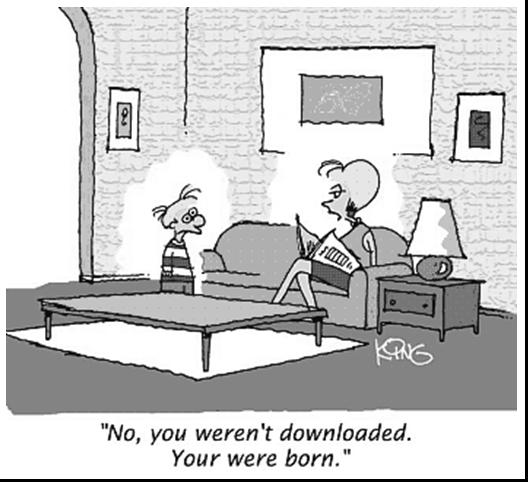
\includegraphics[width=.5\textwidth]{fig1.jpg}
\caption{A typical figure}
\label{fig:exampleFig1}
\end{figure}

\begin{figure}[ht]
\centering
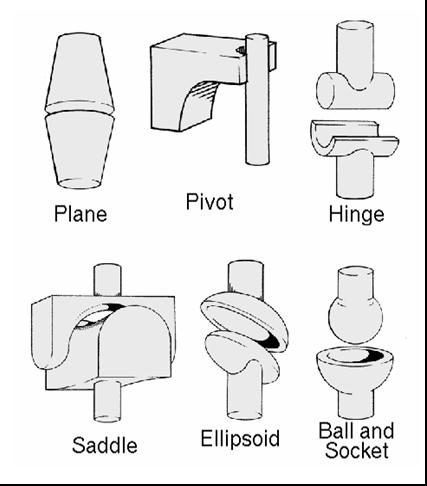
\includegraphics[width=.3\textwidth]{fig2.jpg}
\caption{This figure is an example of a figure caption taking more than one
  line and justified considering margins mentioned in Section~\ref{sec:figs}.}
\label{fig:exampleFig2}
\end{figure}

In tables, try to avoid the use of colored or shaded backgrounds, and avoid
thick, doubled, or unnecessary framing lines. When reporting empirical data,
do not use more decimal digits than warranted by their precision and
reproducibility. Table caption must be placed before the table (see Table 1)
and the font used must also be Helvetica, 10 point, boldface, with 6 points of
space before and after each caption.

\begin{table}[ht]
\centering
\caption{Variables to be considered on the evaluation of interaction
  techniques}
\label{tab:exTable1}
\smallskip
\begin{tabular}{|l|c|c|}
\hline
& Value 1 & Value 2\\[0.5ex]
\hline
&&\\[-2ex]
Case 1 & 1.0 $\pm$ 0.1 & 1.75$\times$10$^{-5}$ $\pm$ 5$\times$10$^{-7}$\\[0.5ex]
\hline
&&\\[-2ex]
Case 2 & 0.003(1) & 100.0\\[0.5ex]
\hline
\end{tabular}
\end{table}

\section{Images}

All images and illustrations should be in black-and-white, or gray tones,
excepting for the papers that will be electronically available (on CD-ROMs,
internet, etc.). The image resolution on paper should be about 600 dpi for
black-and-white images, and 150-300 dpi for grayscale images.  Do not include
images with excessive resolution, as they may take hours to print, without any
visible difference in the result. 

\section{References}

Bibliographic references must be unambiguous and uniform.  We recommend giving
the author names references in brackets, e.g. \cite{knuth:84},
\cite{boulic:91}, and \cite{smith:99}.

The references must be listed using 12 point font size, with 6 points of space
before each reference. The first line of each reference should not be
indented, while the subsequent should be indented by 0.5 cm.

\bibliographystyle{sbc}
\bibliography{sbc-template}

\end{document}
